\chapter{Absolute Value Equations and Inequalities}

\section{Absolute Value Equations}

Solve each of the following.

\begin{multicols}{3}
\begin{enumerate}
	\item $|2x| = 10$
	\item $|3x-7|=8$
	\item $|5x+1| = -4$
\end{enumerate}	\setcounter{Review}{\value{enumi}}
\end{multicols}
\begin{multicols}{3}
\begin{enumerate}	\setcounter{enumi}{\value{Review}}
	\item $|x + 7| = 9$
	\item $|8x+16| = -24$
	\item $|-x-4| = -3$
\end{enumerate}	\setcounter{Review}{\value{enumi}}
\end{multicols}
\begin{multicols}{3}
\begin{enumerate}	\setcounter{enumi}{\value{Review}}
	\item $\left|\frac{1}{2}x + 2\right| = x - 3$
\end{enumerate}	\setcounter{Review}{\value{enumi}}
\end{multicols}



\section{Absolute Value Inequaltiies}

Solve each. Graph your answers on a number line.

\begin{multicols}{3}
\begin{enumerate}
	\item $|x-9| < 10$
	\item $|-x+1| \geq 7$
	\item $|x+8| < -1$
\end{enumerate}	\setcounter{Review}{\value{enumi}}
\end{multicols}
\begin{multicols}{3}
\begin{enumerate}	\setcounter{enumi}{\value{Review}}
	\item $|6x - 18| < 42$
	\item $|-2x+1| \geq 9$
	\item $|5x + 2| < 3x$
\end{enumerate}	\setcounter{Review}{\value{enumi}}
\end{multicols}
\begin{multicols}{3}
\begin{enumerate}	\setcounter{enumi}{\value{Review}}
	\item $|3x + 2| > 1$
    \item $|2x - 1| \leq 7$ 
    \item $|2x-8| \leq 3x$
\end{enumerate}	\setcounter{Review}{\value{enumi}}
\end{multicols}
\begin{multicols}{3}
\begin{enumerate}	\setcounter{enumi}{\value{Review}}
	\item $3\left| \frac{1}{3}x+9\right| > 27$
	\item $|0.1x+5.4| < 4.7$
\end{enumerate}	\setcounter{Review}{\value{enumi}}
\end{multicols}


\newpage

\section{Answer Key}

\subsection*{Absolute Value Equations}

\begin{multicols}{3}
\begin{enumerate}
	\item $x = \pm 5$
	\item $x = -\frac{1}{3} \text{ or } x = 5$
	\item $\emptyset$
\end{enumerate}	\setcounter{Review}{\value{enumi}}
\end{multicols}
\begin{multicols}{3}
\begin{enumerate}	\setcounter{enumi}{\value{Review}}
	\item $x = 2$ or $x = -16$
	\item $\emptyset$
	\item $\emptyset$
\end{enumerate}	\setcounter{Review}{\value{enumi}}
\end{multicols}
\begin{multicols}{3}
\begin{enumerate}	\setcounter{enumi}{\value{Review}}
	\item $x = 10$
\end{enumerate}	\setcounter{Review}{\value{enumi}}
\end{multicols}



\subsection*{Absolute Value Inequalities}

\begin{multicols}{3}
\begin{enumerate}
	\item $-1 < x < 19$ \newline\\
	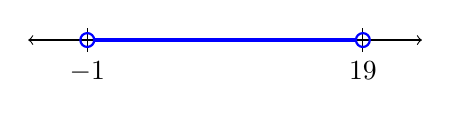
\begin{tikzpicture}
	\draw[<->] (-2.5,0) -- (2.5,0);
	\draw (-1.75,0.15) -- (-1.75,-0.15) node [below] {$-1$};
	\draw (1.75,0.15) -- (1.75,-0.15) node [below] {$19$};
	\draw[very thick, blue, shorten >= 2.5pt, shorten <= 2.5pt] (-1.75,0) -- (1.75,0);
	\draw[blue, thick] (-1.75,0) circle [radius=2.5pt];
	\draw[blue, thick] (1.75,0) circle [radius=2.5pt];
	\end{tikzpicture}
	\item $x \leq -6 \text{ or } x \geq 8$ \newline\\
	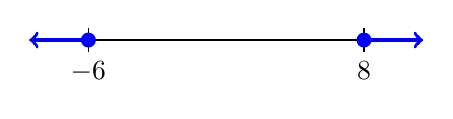
\begin{tikzpicture}
	\draw[<->] (-2.5,0) -- (2.5,0);
	\draw (-1.75,0.15) -- (-1.75,-0.15) node [below] {$-6$};
	\draw (1.75,0.15) -- (1.75,-0.15) node [below] {$8$};
	\draw[very thick, blue, ->] (-1.75,0) -- (-2.5,0);
	\draw[very thick, blue, ->] (1.75,0) -- (2.5,0);
	\draw[blue, fill=blue] (-1.75,0) circle [radius=2.5pt];
	\draw[blue, fill=blue] (1.75,0) circle [radius=2.5pt];
	\end{tikzpicture}
	\item $\emptyset$ \newline\\
	\begin{tikzpicture}
	\draw[<->] (-2.5,0) -- (2.5,0);
	\end{tikzpicture}
\end{enumerate}	\setcounter{Review}{\value{enumi}}
\end{multicols}
\begin{multicols}{3}
\begin{enumerate}	\setcounter{enumi}{\value{Review}}
	\item $-4 < x < 10$ \newline\\
    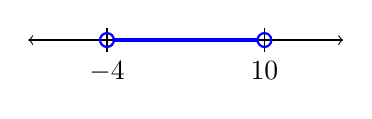
\begin{tikzpicture}
    \draw[<->] (-2,0) -- (2,0);
    \draw (-1,0.15) -- (-1,-0.15) node [below] {$-4$};
    \draw (1,0.15) -- (1,-0.15) node [below] {$10$};
    \draw [very thick, blue, shorten >= 2.5pt, shorten <= 2.5pt] (-1,0) -- (1,0);
    \draw [thick, blue] (-1,0) circle [radius = 2.5pt];
    \draw [thick, blue] (1,0) circle [radius = 2.5pt];
    \end{tikzpicture}  
    \item $x \leq -4$ or $x \geq 5$ \newline\\
    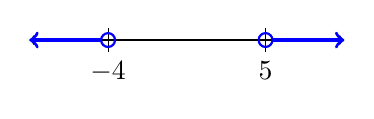
\begin{tikzpicture}
    \draw[<->] (-2,0) -- (2,0);
    \draw (-1,0.15) -- (-1,-0.15) node [below] {$-4$};
    \draw (1,0.15) -- (1,-0.15) node [below] {$5$};
    \draw [->, very thick, blue, shorten <= 2.5pt] (-1,0) -- (-2,0);
    \draw [->, very thick, blue, shorten <= 2.5pt] (1,0) -- (2,0);
    \draw [thick, blue] (-1,0) circle [radius = 2.5pt];
    \draw [thick, blue] (1,0) circle [radius = 2.5pt];
    \end{tikzpicture}
    \item $\emptyset$	\newline\\
    \begin{tikzpicture}
	\draw[<->] (-2.5,0) -- (2.5,0);
	\end{tikzpicture}
\end{enumerate}	\setcounter{Review}{\value{enumi}}
\end{multicols}
\begin{multicols}{3}
\begin{enumerate}	\setcounter{enumi}{\value{Review}}
	\item $x < -1$ or $x > \frac{1}{3}$ \newline\\
    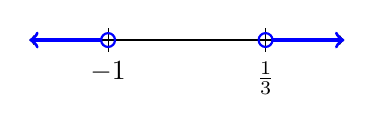
\begin{tikzpicture}
    \draw[<->] (-2,0) -- (2,0);
    \draw (-1,0.15) -- (-1,-0.15) node [below] {$-1$};
    \draw (1,0.15) -- (1,-0.15) node [below] {$\frac{1}{3}$};
    \draw[blue, very thick, ->, shorten <= 2.5pt] (-1,0) -- (-2,0);
    \draw[blue, very thick, ->, shorten <= 2.5pt] (1,0) -- (2,0);
    \draw[thick, blue] (-1,0) circle [radius=2.5pt];
    \draw[thick, blue] (1,0) circle [radius=2.5pt];
    \end{tikzpicture}
    \item $-3 \leq x \leq 4$ \newline\\
    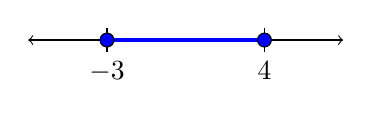
\begin{tikzpicture}
    \draw[<->] (-2,0) -- (2,0);
    \draw (-1,0.15) -- (-1,-0.15) node [below] {$-3$};
    \draw (1,0.15) -- (1,-0.15) node [below] {$4$};
    \draw[blue, very thick] (-1,0) -- (1,0);
    \draw[fill=blue] (-1,0) circle [radius=2.5pt];
    \draw[fill=blue] (1,0) circle [radius=2.5pt];
    \end{tikzpicture}
    \item $x \geq 1.6$ \newline\\
    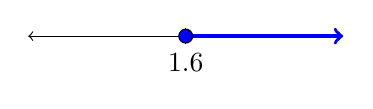
\begin{tikzpicture}
    \draw[<->] (-2,0) -- (2,0);
    \draw (0,0.1) -- (0,-0.1) node [below] {$1.6$};
    \draw[->, blue, very thick] (0,0) -- (2,0);
    \draw[fill=blue] (0,0) circle [radius=2.5pt];
    \end{tikzpicture}
\end{enumerate}	\setcounter{Review}{\value{enumi}}
\end{multicols}
\begin{multicols}{3}
\begin{enumerate}	\setcounter{enumi}{\value{Review}}
	\item $x < -54$ or $x > 0$ \newline\\
    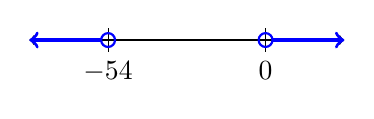
\begin{tikzpicture}
    \draw[<->] (-2,0) -- (2,0);
    \draw (-1,0.15) -- (-1,-0.15) node [below] {$-54$};
    \draw (1,0.15) -- (1,-0.15) node [below] {$0$};
    \draw[->, blue, very thick, shorten <= 2.5pt] (-1,0) -- (-2,0);
    \draw[->, blue, very thick, shorten <= 2.5pt] (1,0) -- (2,0);
    \draw[thick, blue] (-1,0) circle [radius=2.5pt];
    \draw[thick, blue] (1,0) circle [radius=2.5pt];
    \end{tikzpicture}
    \item $-101 < x < -7$ \newline\\
    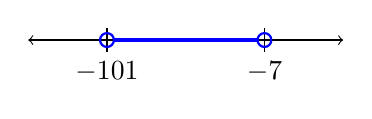
\begin{tikzpicture}
    \draw[<->] (-2,0) -- (2,0);
    \draw (-1,0.15) -- (-1,-0.15) node [below] {$-101$};
    \draw (1,0.15) -- (1,-0.15) node [below] {$-7$};
    \draw[blue, very thick, shorten <= 2.5pt, shorten >= 2.5pt] (-1,0) -- (1,0);
    \draw[thick, blue] (-1,0) circle [radius=2.5pt];
    \draw[thick, blue] (1,0) circle [radius=2.5pt];
    \end{tikzpicture} 
\end{enumerate}	\setcounter{Review}{\value{enumi}}
\end{multicols}


